%******************* START *******************
\documentclass{article}

\usepackage{xcolor}
\usepackage{graphicx}
%\usepackage[numbers]{natbib}
\usepackage{kantlipsum}
\usepackage{tabularray}
\usepackage{booktabs}
\usepackage{cite}
\usepackage{url}

%\citestyle{plain}

\UseTblrLibrary{booktabs}
%\documentclass[12pt,mathdesign]{ndsu-thesis-2022}
%
%
%%-----------------BibTeX-----------------------------------
%\usepackage[numbers,sort&compress]{natbib}
%%\usepackage[numbers]{natbib}
%\citestyle{plain} % agms, agu, arms, egu, cospar, dcu, kluwer, plain, nature
%%\newcommand{\makebib}{\biblio{IEEEtran.bst}{mybib}} 
%\newcommand{\makebib}{\biblio{chicago.bst}{mybib}} % shortcut for bibliography
%
%%-----------------BibLaTeX-----------------------------------
%%\usepackage[style=ieee,natbib=true,backend=biber]{biblatex}% works well with \citep and \citet commands
%%\addbibresource{mybib.bib}% *.bib extension is necessary 
%
%\newcommand\myspacing{1.9}% 23 lines/page needs 1.9 for thesis
%%----------------------------------------------------
%
%\graphicspath{{./figures/}}
%
%\newcommand\makerefs{
%\printbibliography[heading=subbibnumbered, title={References}]
%} % shortcut - section numbered; subbibintoc - unnumbered
%

\title{My NDSU Thesis --- Sandbox}


%************ Document start ************
\begin{document}
\maketitle
%\begin{spacing}{\myspacing}      % New line spacing - 23 lines per page

%----------------------------------------------------
\section{Test Chapter for NDSU Thesis Class Sandbox}

This ``\texttt{ndsu-sandbox.tex}'' file can be used as a sandbox to try out things in the actual NDSU thesis environment. \textcolor{gray}{Things tested here (including the bibliography) can be readily inserted into the original thesis/dissertation document. Therefore, this lightweight source will be convenient to test things out.} So, go for it --- and remember anything is possible by \LaTeX{} (almost!?).

%----------------------------------------------------
\section{Section}
\subsection{Sub-Section}
\subsubsection{Sub-Sub-Section}

\textcolor{gray}{Dummy text from kantlipsum[9]. Reference listing on the next page. Check it for the intended formatting.} I refer to \cite{lamport94,kopka2004guide,baczkowski1990ndsu}. \kant[9] 
\cite{kopka2004guide}, \cite{baczkowski1990ndsu} and \cite{lamport94,kopka2004guide}


\begin{table}[ht]
\centering
\caption{Professional looking fixed-width table using 
\texttt{booktabs} package.}
\begin{tabular}{ l c r }
\toprule
Number & Our rating & Month \\
(left) & (center)   & (right)\\
\midrule
1 & Colder & January \\
2 & Okay   & February \\
3 & Good   & March\\
\bottomrule
\end{tabular}
\label{tab22}
\end{table}

\kant[9]



\begin{table}[h!]
\centering
\caption{Professional looking automatic full-width table using \texttt{tblr} environment and \texttt{booktabs} package.}
\begin{tblr}{X | X[c] | X[r]}
\toprule
Number & Our rating & Month \\
(left) & (center)   & (right)\\
\midrule
1 & Colder & January \\
2 & Okay   & February \\
3 & Good   & March\\
\bottomrule
\end{tblr}
\label{tab25}
\end{table}

\kant[9]

%\myfig{H}{0.4}{frog.jpg}{Figure short caption is centered. Use of myfig command.}{fig2}

\begin{figure}[h!]
\centering
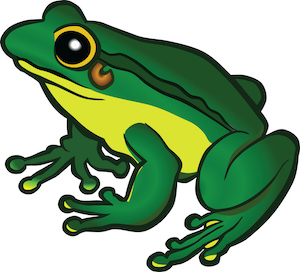
\includegraphics[width=0.4\textwidth]{frog.jpg}
\caption{Our pet frog and has got a caption}
\end{figure}

\kant[9]
%\myfig{H}{0.4}{frog}{Figure short caption is centered. Use of myfig command; Now long caption that will be left-justified.}{fig3}


%----------------------------------------------------
\kant[2-4]
%\makebib % for bibtex
%\makerefs % for biblatex - being first no refsection needed

%----------------------------------------------------
%----------------------------------------------------
\section{Test Second Chapter for NDSU Thesis Class Sandbox}

%\begin{refsection}  % for individual chapter reference (only from this chapter)
\kant[20-21]

%----------------------------------------------------
\section{Section}
\subsection{Sub-Section}
\subsubsection{Sub-Sub-Section}

\textcolor{gray}{Dummy text from kantlipsum. Reference listing on the next page. Check it for the intended formatting.} I refer to \cite{butin2009education}, \cite{rudestam2014surviving, Goossens2008g,cassuto2010advising,pires2021teens}. \kant[9] 

\cite{rudestam2014surviving} found this. \cite{rudestam2014surviving, Goossens2008g,cassuto2010advising}


\bibliographystyle{IEEEtran}%IEEEtranN
\bibliography{mybib.bib}
\end{document}

%******************* END *******************
Option 1
\usepackage[numbers,sort&compress]{natbib}
\bibliographystyle{IEEEtranN}%IEEEtranN

Option 2
\usepackage[sort&compress]{natbib}
\citestyle{plain}
\bibliographystyle{IEEEtranN}%IEEEtranN

Option 3
% Need to spell out authors 
\usepackage[numbers,sort&compress]{natbib}
\bibliographystyle{IEEEtran}%IEEEtran


Option 4
\usepackage[sort&compress]{natbib}
\citestyle{plain}
\bibliographystyle{IEEEtran}%IEEEtran

Option 5 
\bibliographystyle{IEEEtran}%IEEEtran

